\titre{}
\theme{fonctions}
\auteur{Nathan Scheinmann}
\niveau{1M}
\source{}
\type{serie}
\piments{2}
\pts{}
\annee{2425}

\contenu{
	\tcblower
Déterminer l'équation des droites représentées ci-dessous. 
\begin{center}
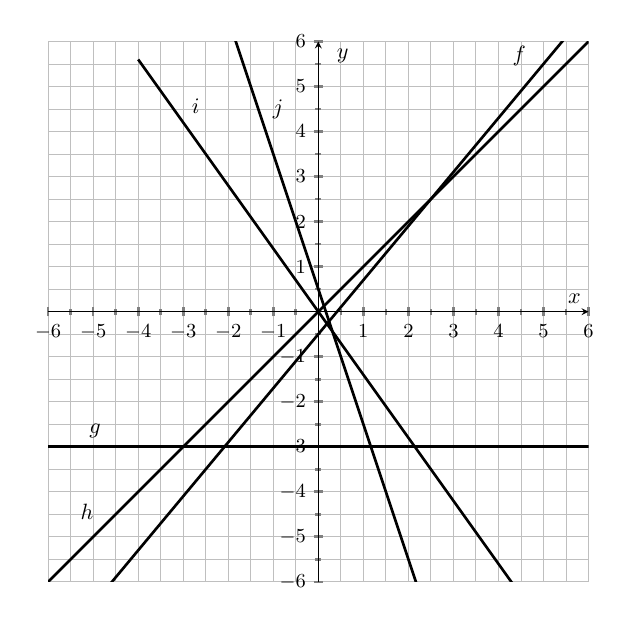
\begin{tikzpicture}[scale=0.8]
\begin{axis}[
  axis lines=center,
  grid=major,
  width=4in,
height=4in,
  xmin=-5,
  xmax=5,
  ymin=-5,
  ymax=5,
  xlabel=$x$,
  ylabel=$y$,
  grid=both,
  minor x tick num=1,
  minor y tick num=1,
  enlargelimits={abs=1},
  xtick={-6,-5,...,6},
  ytick={-6,-5,...,6},
  xlabel style={at={(rel axis cs:1,0.5)}},
  ylabel style={at={(rel axis cs:0.52,1)}},
  tick style={very thick},
  ticklabel style={font=\small},
  legend style={
  at={(rel axis cs:1,1)},
  anchor=north west,
  draw=none,
  inner sep=0pt,
  fill=gray!10}
]

\addplot [very thick,domain=-6:6,samples=200] {6/5*x-0.5} node [above left,pos=0.9] {$f$};
%\addlegendentry {$f(x)=...$};
\addplot[black,very thick,domain=-6:6,samples=200]{-3}  node[above right,pos=0.06] {$g$};
\addplot[black,very thick,domain=-6:6,samples=200]{x}  node[above left,pos=0.1] {$h$};
%\addplot[black,very thick,domain=-6:6,samples=200]{-x+1.5}  node[above right,pos=0.1] {$h$};
%\addplot[black,very thick,domain=-6:6,samples=200]{-0.5*x+0.5}  node[above right,pos=0.1] {$i$};
\addplot[black,very thick,domain=-4:6,samples=200]{-7/5*x}  node[above right,pos=0.1] {$i$};
\addplot[black,very thick,domain=-2:6,samples=200]{-3*x+0.5}  node[above right,pos=0.1] {$j$};
%\addlegendentry{$g(x)=...$};
\end{axis}
\end{tikzpicture}
\end{center}	
}
\correction{
	\tcblower
	\begin{tasks}(6)
		\task[] $y_f=\dfrac{6}{5}x-\dfrac{1}{2}$
		\task[] $y_g=-3$
		\task[] $y_h=x$
		\task[] $y_i=-\dfrac{7}{5}x$
		\task[] $y_j=-3x+\dfrac{1}{2}$
	\end{tasks}

}

